\documentclass{article}
\usepackage{graphicx}
\usepackage{float}
\usepackage{wrapfig}
\usepackage{caption}
\usepackage{subcaption}
\usepackage{booktabs}
\usepackage{array}
\usepackage{enumitem}
\usepackage[table]{xcolor}
\usepackage{amsmath, amssymb}
\usepackage{listings}
\usepackage{algorithm}
\usepackage{algpseudocode}
\usepackage{comment}
\usepackage[numbers]{natbib}
\usepackage{hyperref}
\usepackage{subcaption}
\usepackage{multirow}
\usepackage{amsthm}
\usepackage{minitoc}
\usepackage{authblk}

\newtheorem{proposition}{Proposition}

\title{\textsc{THE SOLAR SYSTEM}}
\author[1]{Johannes Kepler$^1$ \\ $^1$Imperial Matematician, Prague}
\date{July 2026}

\begin{document}

\maketitle
\tableofcontents
\newpage

\section{Our Planetary Neighborhood}

\subsection{The Sun and Its Planets}

The Sun and its gravity-bound bodies form the Solar System\cite{nasa_planets}. See \href{https://science.nasa.gov/solar-system/}{NASA
Solar System Exploration}. In increasing distance, the planets are

Mercury, Venus, Earth, Mars, Jupiter, Saturn, Uranus, Neptune

The planets form two groups:

\begin{enumerate}[label={I}]
    \item \textbf{Inner Planets}
        \begin{itemize}
            \item[$\dagger$] Mercury, Venus, Earth, and Mars belong to this group.
            \item[$\dagger$] They are comparatively small and have solid surfaces.
            \item[$\dagger$]  They are also called the terrestrial planets
        \end{itemize}
    \item \textbf{Outer Planets}
        \begin{itemize}
            \item[$\dagger$] Jupiter and Saturn are gas giants.
            \item[$\dagger$] Uranus and Neptune are commonly called ice giants.
            \item[$\dagger$]  All four outer planets possess ring systems.
        \end{itemize}
\end{enumerate}

\textcolor{red}{The inner planets are small, dense, and relatively close to the Sun}, whereas \textcolor{blue}{the outer planets are much larger and travel along considerably wider orbits.}

\subsection{Portraits of the Solar System}
\ref{fig:fig1} shows the sun and eight planets.
\footnote{Sizes and distances are schematic.}

Compare Mars in \ref{fig:mars} with Jupiter in \ref{fig:jupiter}


\section{Kepler’s Laws of Planetary Motion}
Kepler’s three laws describe planetary motion\cite{nasa_kepler}.
\subsection{First Law: Elliptical Orbits}

A planetary orbit is elliptical, with the Sun at one focus:
\begin{equation}
    \frac{x^2}{a^2} + \frac{y^2}{b^2} = 1, \hspace{20px} a >= b > 0
\end{equation}
Here a and b are the semi-axes.

\begin{figure}[H]
    \centering

    % ==============================
    % Star
    % ==============================
    \textbf{Star}\par\medskip
    \begin{subfigure}{0.4\textwidth}
        \centering
        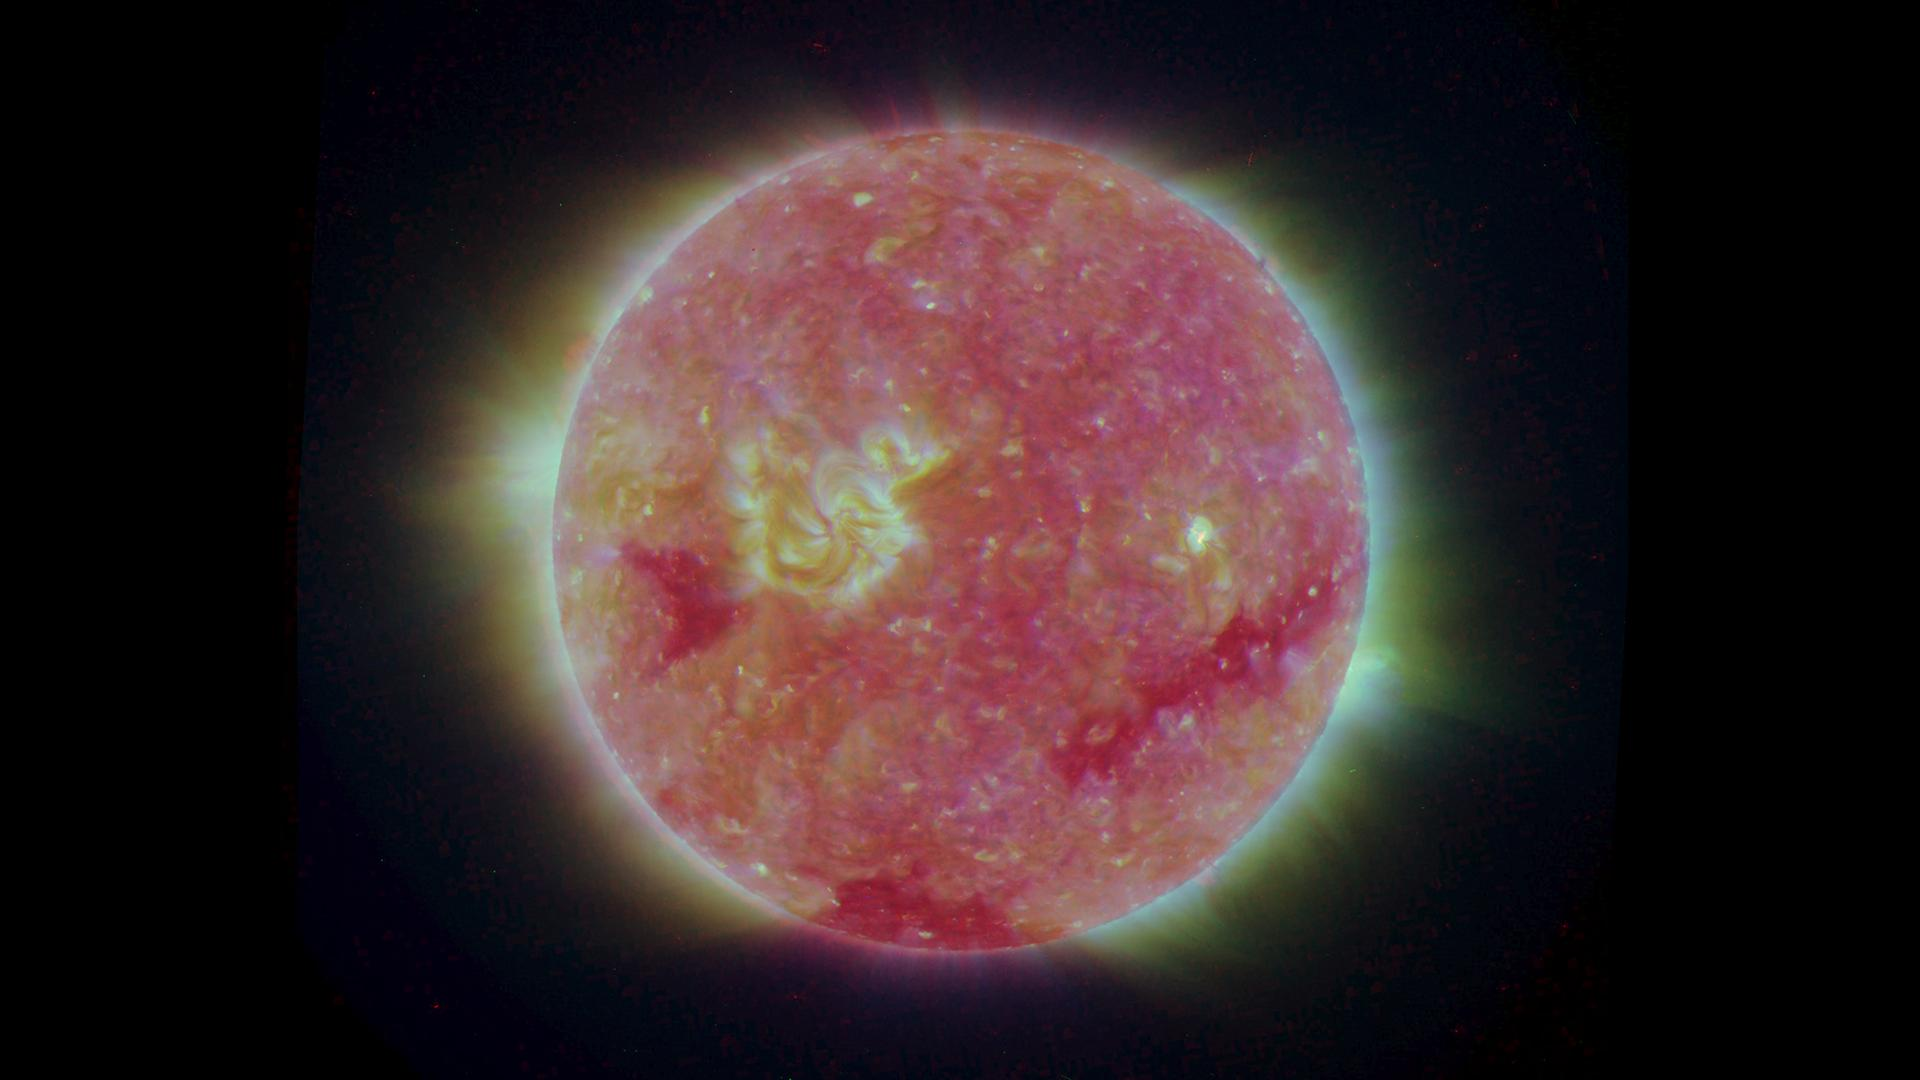
\includegraphics[width=\linewidth]{sun.png}
        \caption{Country scale}
        \label{fig:sub-country}
    \end{subfigure}
    \par\medskip
    \vspace{1cm}
    
    % ==============================
    % Inner Planets (Row 1 of planets)
    % ==============================
    \textbf{Inner Planets}\par\medskip
    \begin{subfigure}{0.2\textwidth}
        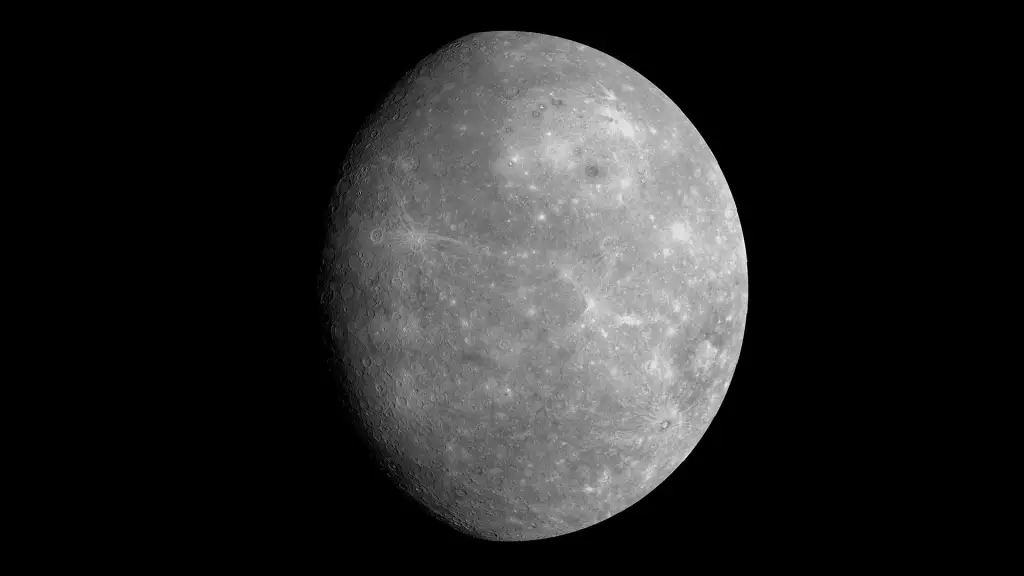
\includegraphics[width=\linewidth]{mercury.png}
        \caption{Mercury}
        \label{fig:mercury} % Fixed duplicate label
    \end{subfigure}
    \hfill
    \begin{subfigure}{0.2\textwidth}
        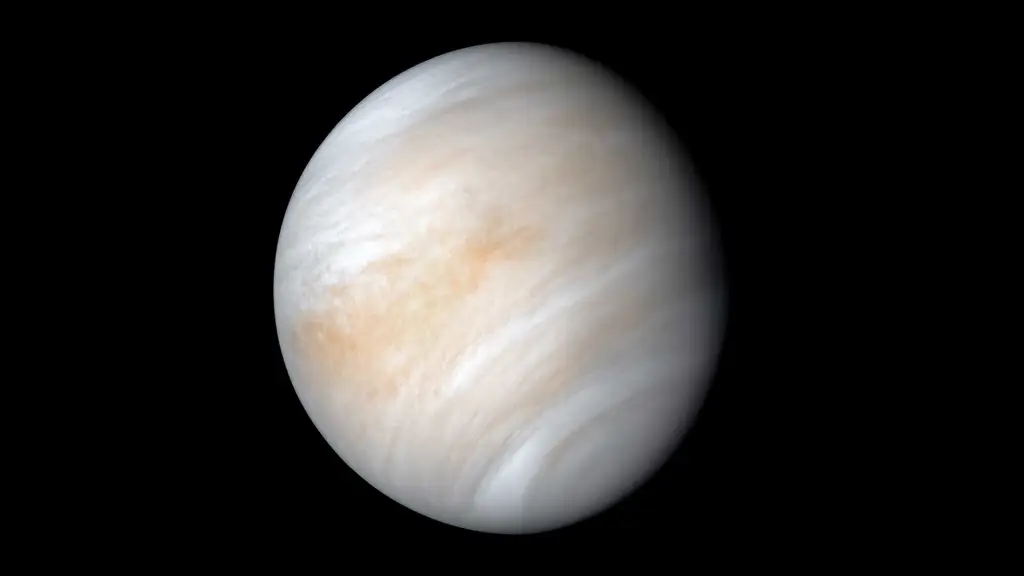
\includegraphics[width=\linewidth]{venus.png}
        \caption{Venus}
        \label{fig:venus}
    \end{subfigure}
    \hfill
    \begin{subfigure}{0.2\textwidth}
        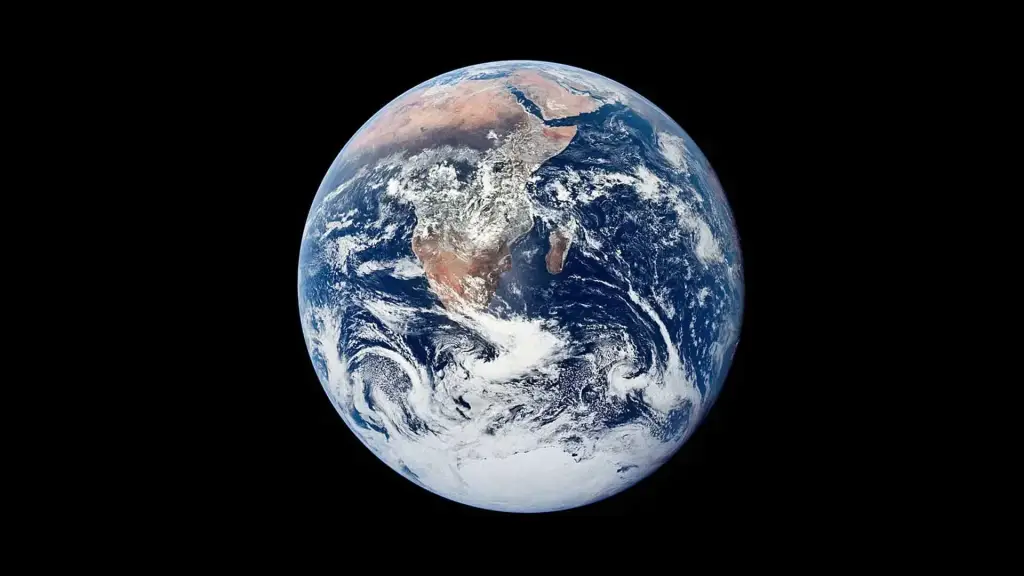
\includegraphics[width=\linewidth]{earth.png}
        \caption{Earth}
        \label{fig:earth}
    \end{subfigure}
    \hfill
    \begin{subfigure}{0.2\textwidth}
        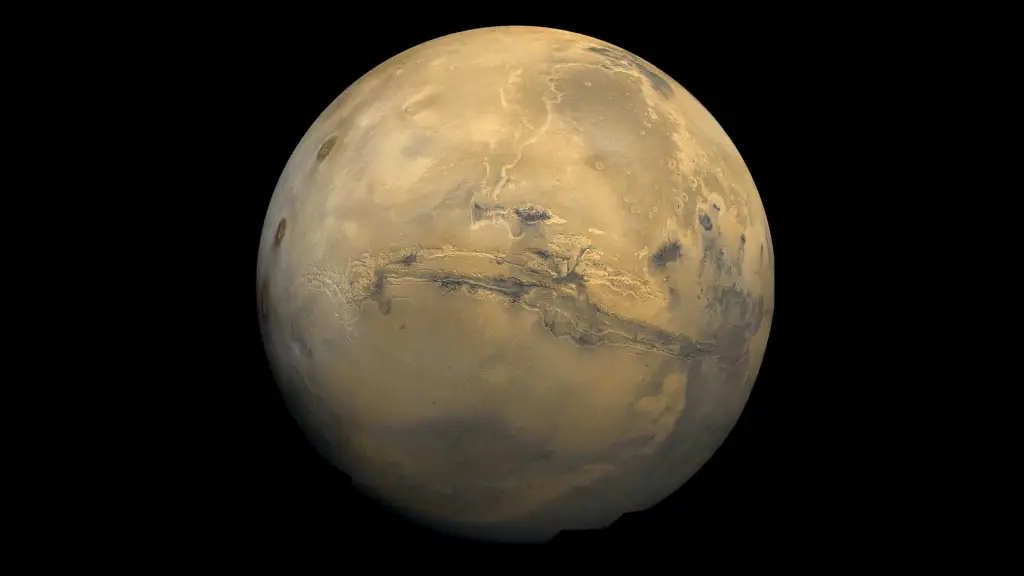
\includegraphics[width=\linewidth]{mars.png}
        \caption{Mars}
        \label{fig:mars}
    \end{subfigure}
    \par\medskip
    \vspace{1cm}
    
    % ==============================
    % Outer Planets (Row 2 of planets)
    % ==============================
    \textbf{Outer Planets}\par\medskip
    \begin{subfigure}{0.2\textwidth}
        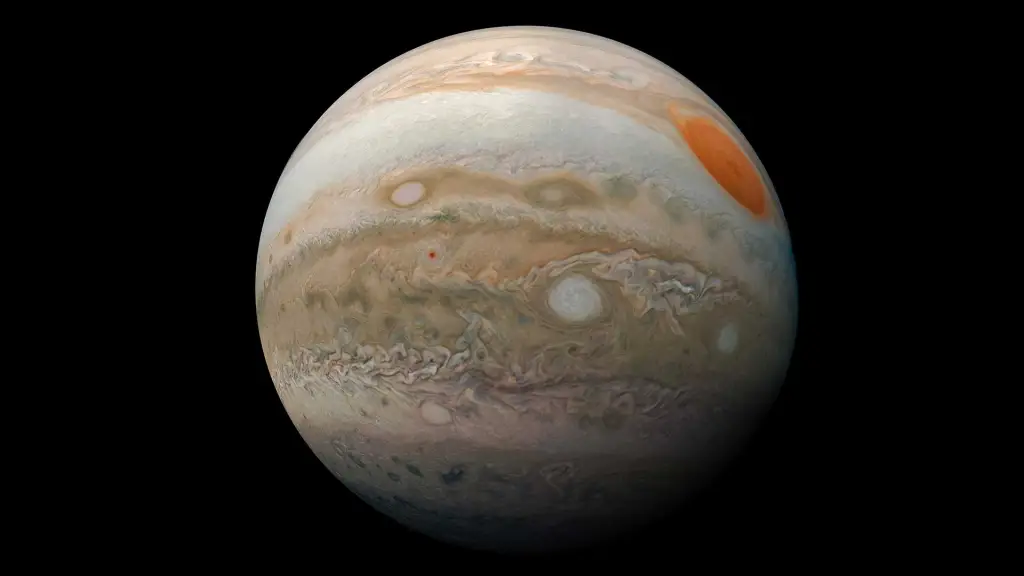
\includegraphics[width=\linewidth]{jupiter.png}
        \caption{Jupiter}
        \label{fig:jupiter}
    \end{subfigure}
    \hfill % Cleaned up the stray backtick here
    \begin{subfigure}{0.2\textwidth}
        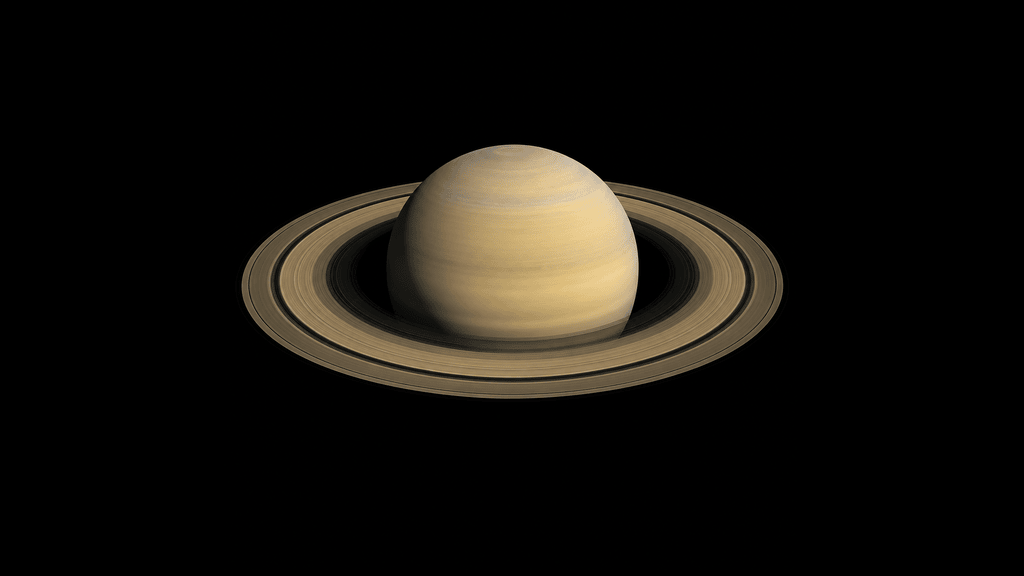
\includegraphics[width=\linewidth]{saturn.png}
        \caption{Saturn}
        \label{fig:saturn}
    \end{subfigure}
    \hfill
    \begin{subfigure}{0.2\textwidth}
        \centering
        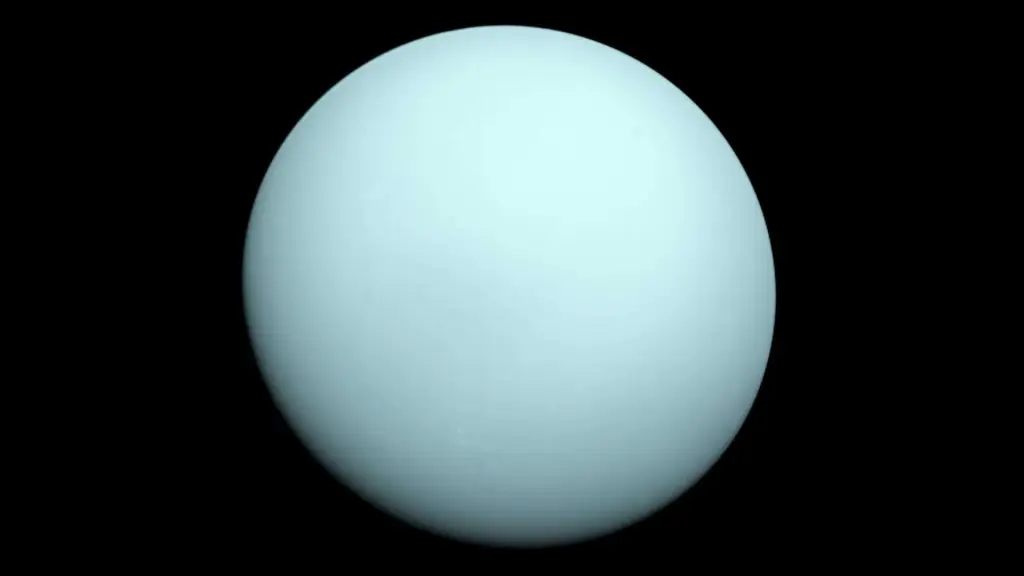
\includegraphics[width=\linewidth]{uranus.png}
        \caption{Uranus}
        \label{fig:uranus}
    \end{subfigure}
    \hfill % Added missing \hfill here
    \begin{subfigure}{0.2\textwidth}
        \centering
        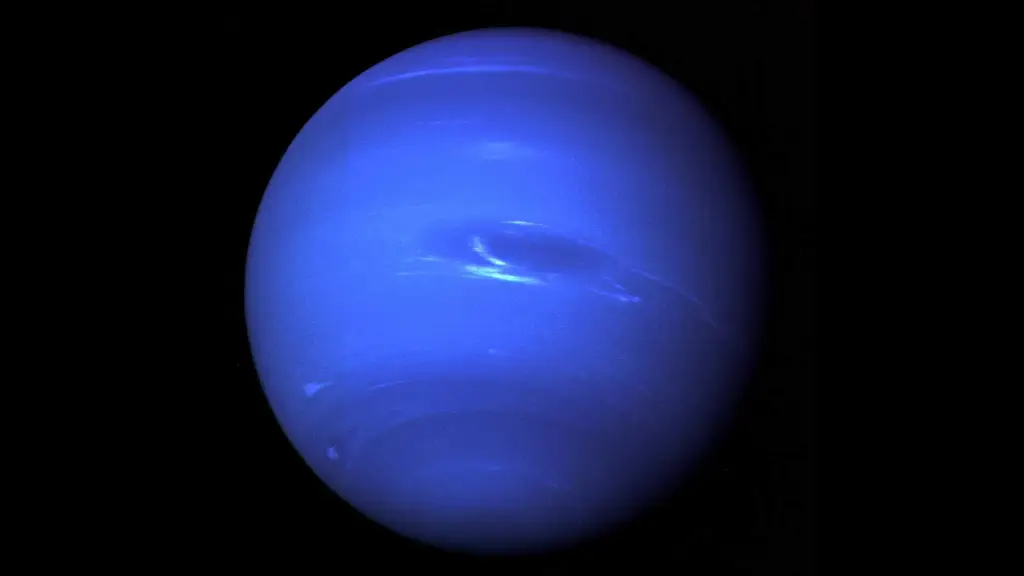
\includegraphics[width=\linewidth]{neptune.png}
        \caption{Neptune}
        \label{fig:neptune}
    \end{subfigure}
    
    \caption{The Sun and the eight planets of the Solar System, arranged into the inner and outer planetary groups. The displayed sizes and distances are not to scale.}
    \label{fig:fig1}
\end{figure}


For focal distance c,
$$
c^2 =  a^2 + b^2
$$
\begin{equation}
    e = \frac{c}{a}
\end{equation}
Here e is the eccentricity.

In polar form,
\begin{equation} \label{eq:eq3}
    r(\theta) = \frac{a(1-e^2)}{1 + e \cos \theta}
\end{equation}

Equation (\ref{eq:eq3}) gives the orbital distance.


\subsection{Second Law: Equal Areas in Equal Times}
Equal times sweep equal areas:
\begin{equation}
\Delta t_1 = \Delta t_2 \implies \Delta A_1 = \Delta A_2 
\end{equation} 

Consequently, a planet moves
\begin{itemize}
    \item[$\diamond$] faster when it is closer to the Sun, and
    \item[$\diamond$] slower when it is farther from the Sun.
\end{itemize}

\subsection{Third Law: Orbital Period and Distance}
For planets orbiting one star,
\begin{equation}
    T^2 \propto a^3.
\end{equation}

Newtonian form:
$$
    T^2 = \frac{4 \pi^3}{GM_{\odot}}a^3,
$$
Here $M_{\odot}$ is the solar mass.

\subsection{An Earth–Mars Comparison}
Using Earth as reference,
$$ a_E = 1 AU \hspace{40px} T_E = 1 \ year$$
where $1 AU \approx 1.496 \times 10^{11}.$ \footnote{AU denotes the mean Earth–Sun distance.} For mars, 
$a_M = 1.524 AU, $ \ so

\begin{equation*}
\begin{split}
\frac{T_M^2}{T_E^2} &= \frac{a_M^3}{a_E^3} \\
T_M &= T_E \left( \frac{a_M}{a_E} \right)^{3/2} \\
&\approx (1.524)^{3/2} \approx 1.88 \text{ years}.
\end{split}
\end{equation*}

Thus $T_M \approx 1.88 \ \text{years}$

\section{A Relativistic Extension}
General relativity extends Kepler’s model.\footnote{Planetary corrections are small but measurable.} Einstein’s equations are
\begin{equation}
    G_{\mu v} + Ag_{\mu v} = \frac{8 \pi G}{c^4} T_{\mu v}
\end{equation}

For spherical mass M,
\begin{equation}
\begin{split}
    ds^2 = - \left( 1 - \frac{r_s}{r} \right) c^2 dt^2 + \left( 1 - \frac{r_s}{r} \right)^{-1} dr^2 \\
    + r^2(d\theta ^2 + \sin ^2 \theta d\phi ^2 ), \hspace{20px} r_s = \frac{2GM}{c^2}
\end{split}
\end{equation}

Free fall satisfies
\begin{equation}
    \frac{d^2 x^\mu}{d\tau ^2} + \Gamma_{\alpha \beta}^{\mu}\frac{dx^\alpha}{d\tau}\frac{dx^\beta}{d\tau} = 0
\end{equation}

Per orbit
\begin{equation}
    \Delta \bar{\omega} = \frac{6\pi GM}{a(1-e^2)c^2} 
\end{equation}
\begin{proposition}[Weak-field circular orbit]
\label{prop:circular}
For a circular orbit of radius $r$,
\begin{equation}
\left( \frac{v}{c} \right)^2 = \frac{GM}{rc^2} = \frac{r_s}{2r}.
\end{equation}
\end{proposition}

\begin{proof}
The circular-orbit balance $v^2/r = GM/r^2$ gives $v^2 = GM/r$. Divide by
$c^2$ and use $r_s = 2GM/c^2$.
\end{proof}

See Proposition~\ref{prop:circular}.
\section{The Outer Planets}
The outer planets are Jupiter, Saturn, Uranus, and Neptune\cite{nasa_temperatures}. The first two
are gas giants; the last two are ice giants.

Table \ref{tab:outer_planets} uses scientific and relativistic notation.\footnote{Values are rounded for typesetting practice}

\begin{table}[H]
\centering
\caption{Orbital parameters and relativistic notation for the outer planets.}
\label{tab:outer_planets}
\renewcommand{\arraystretch}{1.5}
\begin{tabular}{|c|c|c|c|c|}
\hline
\multirow{2}{*}{\textbf{Planet}} & 
\multicolumn{2}{c|}{\textbf{Orbital parameters}} & \multicolumn{2}{c|}{\textbf{Relativistic notation}} \\
\cline{2-5}
& $a$ (AU) & $e$ & $\varepsilon = \dfrac{1}{ac^2}GM_{\odot}$ & $\beta = \sqrt{\varepsilon}$ \\
\hline
Jupiter & 5.204  & $4.89 \times 10^{-2}$ & $1.90 \times 10^{-9}$  & $4.36 \times 10^{-5}$ \\
\hline
Saturn  & 9.583  & $5.65 \times 10^{-2}$ & $1.03 \times 10^{-9}$  & $3.21 \times 10^{-5}$ \\
\hline
Uranus  & 19.191 & $4.72 \times 10^{-2}$ & $5.14 \times 10^{-10}$ & $2.27 \times 10^{-5}$ \\
\hline
Neptune & 30.070 & $8.6  \times 10^{-3}$ & $3.28 \times 10^{-10}$ & $1.81 \times 10^{-5}$ \\
\hline
\end{tabular}
\end{table}

Table \ref{tab:outer_planets} compares the four gas giants


\bibliographystyle{unsrtnat}
\bibliography{main}
\end{document}
